\section[\empty]{The Dataset}



\begin{frame}{Toadstool 2 Dataset}
\begin{block}{}
The dataset consists of video, sensor, and demographic data collected from 10 participants playing a Super Mario Bros.
\end{block}

\vspace{-0.5cm}

		\begin{columns}[T] % Top alignment
		\begin{column}{0.5\textwidth}
			\begin{center}
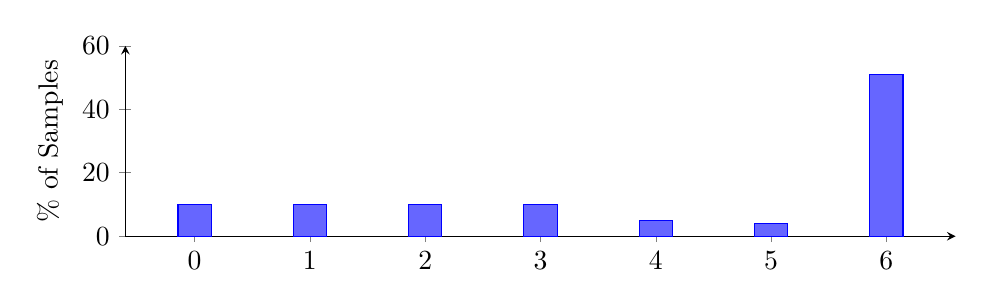
\begin{tikzpicture}
	\begin{axis}[
		width=\textwidth,
		height=4cm,
		ybar,
		bar width=12pt,
		axis x line=bottom,
		axis y line=left,
		ylabel={\% of Samples},
		symbolic x coords={0,1,2,3,4,5,6},
		xtick=data,
%		xticklabel style={rotate=0,anchor=east},
		enlarge x limits=0.1,
		ymin=0, ymax=60
		]
		\addplot+[fill=blue!60] coordinates {
			(0,10) (1,10) (2,10) (3,10) (4,5) (5,4) (6,51)
		};
	\end{axis}
\end{tikzpicture}

  \begin{columns}[t]
	\column{0.33\textwidth}
	\centering\footnotesize
	\begin{tabular}{r l}
		0 & Anger   \\
		1 & Disgust \\
		2 & Fear    
	\end{tabular}
	
	\column{0.33\textwidth}
	\centering\footnotesize
	\begin{tabular}{r l}
		3 & Happy     \\
		4 & Sad       \\
		5 & Surprised 
	\end{tabular}
	
	\column[c]{0.33\textwidth}
	\centering\footnotesize
	\begin{tabular}{r l}
		6 & Neutral\\
		  &  \\
		  &
	\end{tabular}
\end{columns}

			\end{center}
			
		\end{column}
		\begin{column}{0.5\textwidth}
		\centering
		\small
		\begin{tabular}{lcc}
		\toprule
		\textbf{Signal} & \textbf{Rate (Hz)} & \textbf{Channels} \\
		\midrule
		BVP  & 64 & 1      \\
		ACC  & 32 & 3 		\\
		EDA  & 4  & 1      \\
		HR   & 1  & 1      \\
		\bottomrule
		\end{tabular}
		
		\begin{block}{}
			20.970 sensor‐only samples (4 s windows)
		\end{block}

		\end{column}
		
	\end{columns}
\end{frame}


\begin{frame}[t]{Problem Setting}
	\vspace{-2.2em}
	\begin{block}{}
		Let $\{(\boldsymbol{X}^{(i)},\,y^{(i)})\}_{i=1}^N$ be the training dataset, where 
		$\boldsymbol{X}^{(i)}\in\mathcal{X}$ and $y^{(i)}\in\{0,1,\dots,6\}$.  
		Here $\mathcal{X}$ is the space of vector sequences of length $T=256$:
		\[
		\boldsymbol{X}^{(i)}
		= \bigl[\boldsymbol{x}^{(i)}_{1}, \dots, \boldsymbol{x}^{(i)}_{t}, \dots,\boldsymbol{x}^{(i)}_{T}\bigr].
		\]
		$\boldsymbol{x}^{(i)}_{t}$ has $p=6$ elements by channels,
		denoted $x^{(i)}_{t,j}\in\mathbb{R}$ or be a missing value $\hat{x}^{(i)}_{t,j}$.
	\end{block}
	\vspace{-1.5em}

\begin{center}
\begin{tikzpicture}[x=1.5cm,y=1cm]
	\newcommand{\Tmin}{0}   % start of T
	\newcommand{\Tmax}{5}  % end   of T
	\newcommand{\Pdim}{3}   % number of rows (p = 1..Pdim)
	\newcommand{\Ndim}{3}   % number of layers (N = 1..Ndim)
	\newcommand{\Xoff}{0.3}  
	\newcommand{\Yoff}{0.3}  
	
	% Draw each layer N = 1…Ndim (1 is backmost, Ndim is front)
	\foreach \N in {1,...,\Ndim} {
		% how much to shift layer \N back in x,y
		\pgfmathsetmacro{\shift}{0.5*(\Ndim-\N)}
		\begin{scope}[shift={(\shift,\shift)}]
			% for each row p
			\foreach \p in {1,...,\Pdim} {
				% compute its y‐coordinate so p=1 is the top
				\pgfmathtruncatemacro{\y}{\Pdim-\p}
				% and for each time index i
				\foreach \i in {\Tmin,...,\Tmax} {
					% pattern: one blue then (p-1) reds
					\pgfmathtruncatemacro{\modres}{mod(\i,\p)}
					\ifnum\modres=0
					\def\fillcolor{MyAccent!20}
					\def\labeltext{$x_{\i,\p}^{(\N)}$}
					\else
					\def\fillcolor{red!20}
					\def\labeltext{$\hat x_{\i,\p}^{(\N)}$}
					\fi
					\fill[fill=\fillcolor,draw=MyDarkBlue]
					(\i,\y) rectangle ++(1,1);
					\node[text=black,font=\footnotesize]
					at (\i+0.5,\y+0.5) {\labeltext};
				}
			}
		\end{scope}
	}
	
	% ─────── Braces ─────────────────────────────────────────────
	% T‐brace above, spanning all time‐cells:
	\draw[decorate,decoration={brace,amplitude=4pt}]
	(\Tmin,\Pdim+\Yoff) -- (\Tmax+1,\Pdim+\Yoff)
	node[midway,above=4pt] {$T$};
	
	% p‐brace at right, spanning all rows:
	\draw[decorate,decoration={brace,amplitude=4pt,mirror}]
	(\Tmax+1+\Xoff,0) -- (\Tmax+1+\Xoff,\Pdim)
	node[midway,right=4pt] {$p$};
	
	% N‐brace (diagonal) from front layer to back layer:
	\pgfmathsetmacro{\Nshift}{0.5*(\Ndim-1)}
	\pgfmathsetmacro{\startX}{\Tmin-\Xoff}
	\pgfmathsetmacro{\startY}{\Pdim}
	\pgfmathsetmacro{\endX}{\Tmin+\Nshift-\Xoff}
	\pgfmathsetmacro{\endY}{\Pdim+\Nshift}
	\draw[decorate,decoration={brace,amplitude=4pt}]
	(\startX,\startY) -- (\endX,\endY)
	node[midway,above left=2pt] {$N$};
\end{tikzpicture}
\end{center}

\end{frame}



